\chapter[Bespreking]{Bespreking}
\label{chap_bespreking}

Dit hoofdstuk zal uit de meeste onderdelen bestaan. Hier wordt het volledig gepresteerde werk beschreven, inclusief korte theoretische beschrijving (indien relevant. 
Vervolgens volgt een gedetailleerde beschrijving van hoe je tot het eindproduct bent gekomen, welke problemen je bent tegengekomen, hoe je ze hebt opgelost, etc.

De titel van dit hoofdstuk zal meestal als volgt uit zien: 'Bespreking [titel]'. Neem hierbij een (kortere) werktitel van je project, bijvoorbeeld: "Bespreking CRM project" of "Bespreking super-geleidende voltaische cel"

Dit hoofdstuk mag enkel flarden computer-code bevatten. Volledige source-code kan eventueel als appendix toegevoegd worden indien relevant en enkel met toestemming van de promotor.

Mogelijke onderdelen kunnen onder andere zijn:
\begin{itemize}
  \item Inleiding probleem (bestaand onderzoek/producten) 
  \item Functionaliteit van eigen product (algemeen overzicht)
  \item Architectuur van eigen product
  \item Bespreking aparte componenten/blokken (problemen + oplossingen)
  \item Bespreking werking van componenten samen
\end{itemize}


In dit hoofdstuk kan je een aantal voorbeelden van vaak voorkomende \LaTeX\ features terugvinden.

\section{Refereren}

Het is mogelijk om met enkele eenvoudige commando's binnen uw tekst te refereren naar chapters, sections of figuren. 

Zo beschrijven we in hoofdstuk \ref{chap_besluit} op pagina \pageref{chap_besluit} wat we verwachten van een goed besluit en hebben we op pagina \pageref{fig_voorbeeld1} een voorbeeldfiguur geplaatst.  

Op pagina \pageref{eq:polynoom} staat een voorbeeld van een wiskundige formule.

De rode kaders zijn steeds klikbaar, maar ze worden niet mee afgedrukt op papier.

\section{Bibliografie}

Om te verwijzen naar een boek, artikel, website of een andere nuttige bron maken we gebruik van de bibliografie.
Het opnemen van artikels in de bibliografie geeft de persoon die uw tekst leest de mogelijkheid om meer informatie op te zoeken als er bepaalde zaken zijn die niet volledig worden uitgewerkt of toegelicht binnen uw scriptie.
De gegevens die in de bibliografie terecht komen worden uit het bestand ``bibliografie.bib'' gehaald. 

Om een nieuw item aan de bibliografie toe te voegen moet je dus twee zaken doen:

\begin{enumerate}
 \item De benodigde informatie toevoegen aan het .bib bestand
 \item Ergens binnen uw tekst verwijzen naar dit item met het ``cite'' commando.
\end{enumerate}

Hier is een voorbeeld van een verwijzing naar de bibliografie \cite{GridCast2} en dit is er ook \'e\'en \cite{gridrm}.

Ook hier zijn de groene kaders weer klikbaar en worden ze niet mee afgedrukt op papier.

De inhoud van de bibliografie zou vergelijkbaar moeten zijn met de informatie die je op onderstaande website kan vinden.

Harvard Referencing for Electronic Sources, \url{http://www.lc.unsw.edu.au/onlib/ref_elec1.html#elec10}

\subsection{Plaatsing verwijzingen naar bibliografie}

\textit{Ik heb nog een vraag over het refereren. Is het de bedoeling dat de referentie in het begin of op het einde van de tekst (alinea) staat?}

Geen \'e\'en van de twee, het moet op de juiste plek staan.
Plaats verwijzingen naar de bibliografie op de juiste plek, dus niet steeds op het einde van een alinea.

Mooi voorbeeld van uit de scriptie van 2012:

De WRAP 920AR is in de verkoop gegaan in januari 2010, maar hij is nog steeds \'e\'en van de beste 
die er te koop is [1]. 
Deze bril kan als een gewone bril opgezet worden. Er komen wel meteen enkele praktische
nadelen bij kijken [2]. Ten eerste steken linkeroor 2 kabels naar buiten, waardoor de bril scheef
komt te staan op je hoofd. De kabels hebben de volgende functie: de eerste kabel stuurt de
webcam aan en is overbodig als de gebruiker alleen de displays wilt gebruiken. De tweede kabel
is verbonden met een afstandsbediening die dan op zijn beurt verbonden is met een USB-poort
en een VGA-poort. De USB-verbinding is nodig om de sensoren uit te lezen en de bril te
voorzien van stroom. De VGA-poort stuurt de 2 displays aan die in Windows herkend worden
als 1 extern scherm [3]. Het tweede nadeel is dat de elektronica dicht tegen het voorhoofd van de
gebruiker zit wordt, wat na een tijd begint te irriteren door de warmte ontwikkeling [4].

Bij iedere referentie verwacht je als lezer iets anders, het is belangrijk dat je als schrijver uw referenties op de juiste plek zet.

\begin{itemize}
 \item $[1]$: info over de huidige markt, prijzen en specificaties
 \item $[2]$: artikel over de nadelen
 \item $[3]$: herkenning van bril in Windows
 \item $[4]$: hier verwacht ik een referentie over irraties
\end{itemize}

\section{Afbeeldingen}

Als je afbeeldingen invoegt, denk er dan aan dat deze voldoende van kwaliteit moeten zijn.

In afbeelding \ref{fig_voorbeeld1} zie je een afbeelding met een te lage resolutie. Afbeelding \ref{fig_voorbeeld2} ziet er al beter uit omdat deze figuur een hogere resolutie heeft.

Bij inzoomen of bij afdrukken zal figuur \ref{fig_voorbeeld3} toch nog iets hoger van kwaliteit zijn omdat dit een vectori\"ele afbeelding is. 
Standaard is ondersteuning voor .pdf en .eps vectorafbeeldingen voorzien.

\begin{center}
  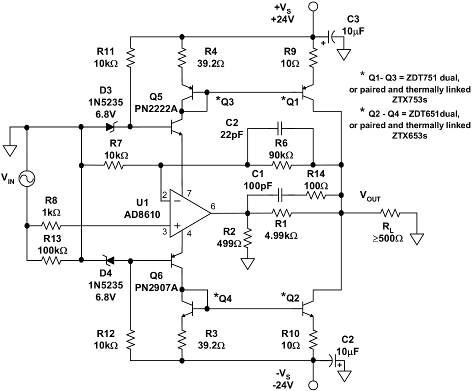
\includegraphics[width=0.95\textwidth]{figures/chap2/schema.png}
  \captionof{figure}[Schema met een te lage resolutie22]{Schema met een te lage resolutie
  \label{fig_voorbeeld1}}
\end{center}

\begin{center}
  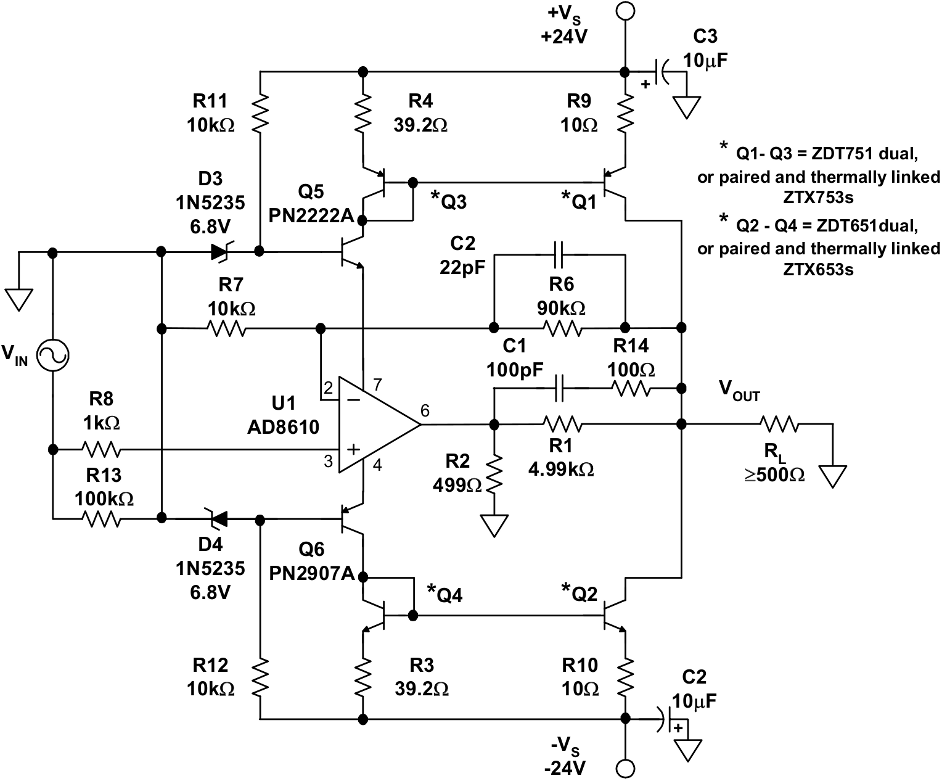
\includegraphics[width=0.95\textwidth]{figures/chap2/schema2.png}
  \captionof{figure}[Schema met een hogere resolutie]{Schema met een hogere resolutie
  \label{fig_voorbeeld2}}
\end{center}

\begin{center}
\includegraphics[width=0.95\textwidth]{figures/chap2/schema2.pdf}
\captionof{figure}[Schema als een vectori\"ele afbeelding]{Schema als een vectori\"ele afbeelding\label{fig_voorbeeld3}}
\end{center}

\section{Tabellen}

De meest elementaire tabel geeft het volgende resultaat:

\begin{tabular}{ l c r }
  1 & 2 & 3 \\
  4 & 5 & 6 \\
  7 & 8 & 9 \\
\label{eenvoudige tabel}
\end{tabular}

Meer geavanceerde tabellen zijn iets moeilijker om te defini\"eren, maar als je op internet zoekt naar andere voorbeelden, die je kan overnemen en aanpassen zodat je bekomt wat je in gedachten had.

Een tabel met redelijk veel tekst die gecentreerd wordt weergegeven.

\begin{center}
    \begin{tabular}{ | l | l | l | p{5cm} |}
    \hline
     Day         & Min Temp & Max Temp & Summary \\ \hline \hline
     Monday      & 11C      & 22C      & A clear day with lots of sunshine.  
     However, the strong breeze will bring down the temperatures. \\ \hline
     Tuesday     & 9C       & 19C      & Cloudy with rain, across many northern regions. Clear spells across most of Scotland and Northern Ireland, but rain reaching the far northwest. \\ \hline
     Wednesday   & 10C      & 21C      & Rain will still linger for the morning. Conditions will improve by early afternoon and continue throughout the evening. \\
    \hline
    \end{tabular}
\label{tb:Xname}
\end{center}

Een iets complexere tabel die aan de linkerrand van de pagina wordt weergegeven.

\begin{flushleft}
\begin{tabular}{|l|l|l|}
\hline
\multicolumn{3}{|c|}{Leeds United: 2003-2004} \\
\hline
 Goalkeeper                  & GK  & Paul Robinson \\ \hline
\multirow{4}{*}{Defenders}   & LB  & Lucus Radebe \\
                             & DC  & Michael Duberry \\
                             & DC  & Dominic Matteo \\
                             & RB  & Didier Domi \\ \hline
\multirow{3}{*}{Midfielders} & MC  & David Batty \\
                             & MC  & Eirik Bakke \\
                             & MC  & Jody Morris \\ \hline
Forward                      & FW  & Jamie McMaster \\ \hline
\multirow{2}{*}{Strikers}    & ST  & Alan Smith \\
                             & ST  & Mark Viduka \\
\hline
\end{tabular}
\end{flushleft}

\section{Formules}

De mogelijkheden om formules in te voegen zijn \'e\'en van de sterkste punten van \LaTeX. 
Het vraagt in het begin wat moeite om de syntax onder de knie te krijgen, maar door intelligent gebruik te maken van de ``alternative text'' velden van wikipedia kan je heel snel formules opstellen.
(alle formules die je op Wikipedia terugvindt zijn namelijk ook met latex commando's geschreven.

Onderstaande formules geven een voorbeeld. Deze formules hebben ook een label, en ze worden automatisch genummerd, bijgevolg kan je er ook in je tekst op een dynamische manier naar verwijzen.

Voorbeeld: ``De Wet van Amp\`ere met Maxwell-correctie staat uitgeschreven in formule \ref{eq:maxwell} op pagina \pageref{eq:maxwell}.''

\begin{equation} \label{eq:polynoom}
x^2 - 5 x + 6 = 0
\end{equation}

\begin{equation} \label{eq:maxwell}
\oint_{\partial S} \mathbf{H} \cdot \mathrm{d}\mathbf{l} = I_{f,S} + \frac {\partial \Phi_S(\mathbf D)}{\partial t} 
\end{equation}

Je kan ook binnen een lopende tekst een formule toevoegen. Dit doe je door uw formule tussen twee dollartekens te plaatsen zoals ik hier doe $i \hbar {\partial \over \partial t} \Psi(x,\,t)= -{\hbar^2  \over 2m} {\partial^2 \over \partial x^2} \Psi(x,\,t)+ V(x)\Psi(x,\,t)\,$. Het is niet mogelijk om naar deze formule te verwijzen omdat er geen label aan werd toegekend.


\section{Packages}
Om extra functionaliteit toe te voegen aan het standaard \LaTeX systeem kan de gebruiker packages toevoegen. Dit is in die sjabloon reeds gedaan in het header.tex bestand.

Als je zelf extra packages wil toevoegen, doe dit dan steeds in overleg met je promotor. Sommige packages kunnen namelijk voor te grote veranderingen van de opmaak van het document zorgen.


\subsection{TODO}

Deze package laat het snel toevoegen van inline opmerkingen toe.
Het plaatsen van een opmerking gebeurt met het ``TODO[tekst]'' commando.
De tekst tussen [..] wordt opgenomen in het .pdf bestand en er wordt een apart .TODO bestand aangemaakt. 
In dit bestand krijg je een compact overzicht van alle ``todos'' in het volledige document.

\TODO[voorbeeld van een todo]

Deze package heeft drie mogelijk modi:

Standaard modus: weergaven van TODO zoals in bovenstaand voorbeeld
\begin{verbatim}
 \usepackage[final]{sty/TODO}
\end{verbatim}

Final modus: als er nog een todo in de tekst staat zal dit een error geven zodat je niet per ongeluk een ``final'' document kan afgeven met de TODO label er nog in.
\begin{verbatim}
 \usepackage[final]{sty/TODO}
\end{verbatim}

Silent modus: in deze modus worden de TODO label onderdrukt. 
Je kan dus een propere tekst genereren zonder al de TODO te moeten wissen of in commentaar te zetten. 
Dit kan nuttig zijn om een propere tussentijdse versie van uw scriptie aan te maken.
\begin{verbatim}
 \usepackage[silent]{sty/TODO}ackage 
\end{verbatim}

\section{Lijsten}

Er zijn een aantal manieren om lijsten te defini\"eren. Probeer steeds gebruik te maken van de de meest logische variant.

Een genummerde lijst (itemize)

\begin{itemize}
  \item Deze zaken
  \item staan in een
  \item lijst die genummerd is
\end{itemize}

Ongenummerde lijst met kleine interlinie (enumerate*)

\begin{enumerate*}
  \item Een element
  \item Nog een element
  \item Weer een element
\end{enumerate*}

Ongenummerde lijst met grotere interlinie (enumerate)

\begin{enumerate}
  \item Een element
  \item Nog een element
  \item Weer een element
\end{enumerate}

Ongenummerde lijst met key topics in het vet, voornamelijk gebruikt als je een lijst hebt waarin je de bullets ook wil omschrijven (description)

\begin{description}
  \item [Water] noodzakelijke voorwaarde voor de meeste levensvormen
  \item [Aarde] de bodem waarop de meeste planten zich vasthechten
  \item [Vuur] handig om de smaak van vlees te verbeteren
\end{description}



\section{Titels}

Bij het kiezen van de titels van hoofdstukken zijn er twee zaken die je kan instellen.

Bijvoorbeeld:

\begin{verbatim}
  \chapter[Ohm en Kirchoff]{De wetten van Ohm en Kirchoff}
\end{verbatim}

Hier zal de tekst \texttt{De wetten van Ohm en Kirchoff} gebruikt worden als titel bij het hoofdstuk in kwestie.

De tekst \texttt{Ohm en Kirchoff} zal echter gebruikt worden in de inhoudstabel, in de ``navigation sidebar'' van je pdf reader en als hoofdstuk aanduiding bovenaan iedere pagina.

\section{Spellingscontrole}

Maak gebruik van spellingscontrole wanneer je aan uw scriptie werkt.

De meeste degelijke \LaTeX\ editors hebben een ingebouwde spellingscontrole.
Moest je gebruik maken van een editor die niet over deze feature beschikt controleer uw source bestanden toch op een andere manier op spelfouten.

\section{Broncode invoegen}

Dit kan je relatief proper met de listing package.

Voorbeeld:

\lstset{numbers=left, stepnumber=1, basicstyle=\footnotesize, language=C++, caption=AcceleroDice: Minimal Implementation, label=AcceleroDice, frame=none, xleftmargin=.3in}
\lstinputlisting{chapters/dice2.pde}

\section[taal]{Taalgebruik}

\TODO[Nog verder toelichten]

\subsection{Notatie SI eenheden}

Spatie tussen eenheid en grootheid voor SI eenheden: \url{http://www.eng-tips.com/viewthread.cfm?qid=111559}


\subsection{Etcetera}
Zet geen ``...'' of ``etc'' in uw tekst, dit doe je enkel in een chat of als je te lui bent om de volledige lijst op te zoeken

\url{http://grammarist.com/usage/et-cetera-etc}


\subsection{Zekerheden en twijfel}

Deze versie zou moeten werken onder Android en iOS.

Zeg ofwel: volgens de datasheet... volgens de specificatie...

Ofwel test iets voor je het zegt of meet het na


\subsection{Begin van een alinea}
``Voor de juiste positiebepaling van de marker zal ik eerst uitleggen hoe een camera (en oog) een 3D-wereld ziet.''
Vanop een bepaald punt (0,0,0) kijkt de camera in de diepte. Hoe verder er in de diepte wordt
gekeken hoe meer ook rechts en links alles zichtbaar wordt...

Zeg niet ``ik ga dit doen'', ``ik zal dat uitleggen'', leg het gewoon uit. Die eerste zin kan dus volledig geschrapt worden.

Een inleiding in het begin van een hoofdstuk om de structuur van het hoofdstuk te schetsen is uiteraard wel toegestaan.


